\documentclass[a4paper]{article}

%% Language and font encodings
\usepackage[english]{babel}
\usepackage[utf8x]{inputenc}
\usepackage[T1]{fontenc}

%% Sets page size and margins
\usepackage[a4paper,top=3cm,bottom=2cm,left=3cm,right=3cm,marginparwidth=1.75cm]{geometry}

%% Useful packages
\usepackage{amsmath}
\usepackage{amsfonts}
\usepackage{graphicx}
\usepackage[colorinlistoftodos]{todonotes}
\usepackage[colorlinks=true, allcolors=blue]{hyperref}
\usepackage{algorithm}
\usepackage{algpseudocode}
\usepackage[lofdepth,lotdepth]{subfig}
\usepackage{graphicx}
\title{Report}
\author{Shagadatov Nurlan}
\newcommand*{\argmin}{\operatornamewithlimits{arg\,min}}
\begin{document}
\maketitle

\section{Variance reduced estimator}

\begin{equation*}
f(X_p) = \mathbb{E} \left[ f(X_p)|\zeta_j \right] + \sum_{k\in \mathbb{N}_0^d \setminus \left\{ 0\right\}} \sum_{l=j+1}^p a_{p,l,k} (X_{l-1})\mathbf{H_k}(Z_l),
\end{equation*}
\begin{equation*}
a_{p,l,k} (x) = \mathbb{E} \left[ f(X_p) \mathbf{H_k}(Z_l) | X_{l-1} = x\right]
\end{equation*}

\begin{align}
M_{K,n}^N(f) & =\sum_{\mathbf k\colon 0<\|\mathbf{k}\|\le K}\sum_{p=N+1}^{N+n}\omega_{p,n}^{N}\sum_{l=N+1}^{p}a_{p,l,\mathbf{k}}(X_{l-1})\mathbf{H}_\mathbf{k}(Z_{l})
\label{eq:29032018a5}\\
&=\sum_{\mathbf k\colon 0<\|\mathbf{k}\|\le K}\sum_{l=N+1}^{N+n}\bar{a}_{l,\mathbf{k}}(X_{l-1})\mathbf{H}_\mathbf{k}(Z_{l})
\notag
\end{align}
with \(\|\mathbf{k}\|=\max_{i} k_i\) and


\begin{equation*}
\pi_{K,n}^N(f) = \pi_n^N(f) -  M_{K,n}^N(f) \\
\end{equation*}

\section{Algorithm 1}
The coefficients \(a_{p,l,k}\)  can be alternatively represented as 
\begin{eqnarray*}
a_{p,l,k}(x)=\mathbb{E} \left[ \mathbf{H}_\mathbf{k}( \xi ) Q_{p,l}(x - \gamma_{l} \mu (x) + \sqrt{\gamma_{l}}\xi)\right]
\end{eqnarray*}
with \(Q_{p,l}(x)=\mathbb{E}\left[\left.f(X_{p})\right|X_{l}=x\right].\) 
On the other hand, due to (almost) time-homogenous markov chain generated by ULA, functions $Q_{p,l}$ can be approximated via regression depending only on number of lags $p-l$:

\[ Q_{p,l}(x) = \mathbb{E} \left[f(X_p) | X_l = x\right] = G_{p-l}(x) = \mathbb{E} \left[ f(\varPhi ^{p-l} (x, \xi))\right]\]

Thus we have:

\[ \forall l: \quad G_r(x) = \mathbb{E} \left[f(X_{l+r}) | X_l = x \right]\]

Consequently, functions $G_r$ could be estimated using regression:

\[ \hat{G}_r = \argmin_{\psi \in \Psi} \sum_{s = 1}^{N_{train}} \sum_{l = N + 1}^{N+n-r} \left| f(X_{l+r}^{(s)}) - \psi(X_l^{(s)})\right|^2 \] 

where $\quad  1 \leq r \leq n-1$ and $\hat{G}_0(x) = f(x)$

\textbf{Lemma (decay of coefficients).}	
Suppose that \(f,\mu\in C^1(\mathbb{R}),\) \(0<b_\mu\leq \mu'(x)\leq B_\mu\) and \(B_\mu\gamma_{l}\leq 1,\) then
\begin{eqnarray*}
\|a_{p,l,\mathbf{k}}\|_{\infty}\leq \sqrt{\gamma_l}\, \|f'\|_\infty\exp\left(-b_{\mu}\sum_{r=l+1}^p \gamma_{r}  \right),\quad \mathbf{k}\in \mathbb{N}^d\setminus \{\mathbf{0}\}
\end{eqnarray*}


Therefore, we can reduce number of estimations by approximation $Q_{p,l}$ for $p-l < \tilde{n}(U,d)$. It allows us to construct small amount of training trajectories (and even use only target trajectory) to approximate conditional expectations $Q_{p,l}$. 

Eventually, we have truncated version of algorithm to compute variance reduced estimator:

\[ \pi_{K,n}^N(f) = \pi_n^N(f) -  M_{K,n, \tilde{n}}^{N}(f)\]

where 

\[{\widehat  M}_{K,n, \tilde{n}}^N = \sum_{0<\left\| k\right\| \leq K} \sum_{p=N+1}^{N+n} \omega_{p,n}^N
\sum_{l=N+1}^p {\widehat  a}_{p,l,k}(X_{l-1})\mathbf{H_K}(Z_l) \mathbb{I}\{ p-l < \tilde{n} \} \]

\subsection{Polynomial approximation}
In order to compute coefficients $a_{p,l,k}$ we need to compute expectations according to distribution of $Z_l$. This could be done by fast integration methods, such as FFT. On the other hand, in case of ULA we can derive explicit formula using polynomial approximation for $Q_{p,l}$.
Suppose we constructed a polynomial approximation  for \(Q_{p,l}(x) \)  of the form:
\begin{eqnarray*}
\widehat Q_{p,l}(x) = \sum_{\|\mathbf{s}\|\leq m} \beta_{\mathbf{s}} x^{\mathbf{s}},\quad s=(s_1,\ldots,s_d)
\end{eqnarray*}
for some \(\beta_{\mathbf{s}}\in \mathbb{R}.\)
Then using the identity
\begin{eqnarray*}
\xi^j = j! \sum_{r = 0}^{j/2} \frac{1}{2^r  r! \sqrt{(j-2r)!}} H_{j-2r}(\xi),\quad \xi \in \mathbb{R},
\end{eqnarray*}
we derive
\begin{eqnarray*}
\widehat a_{p,l,\mathbf{k}} (x) &=&\mathsf{E} \left[ \mathbf{H}_\mathbf{k}(x) Q_{p,l}(x - \gamma \mu(x) + \sqrt{\gamma}\xi)\right] =
\\
%&=&  \mathsf{E} \left[\prod_{i=1}^d H_{k_i}(\xi_i) \cdot \left(\sum_{t_1=0, \dots, t_d=0}^{max_k(t_k) \leq m} \beta_{t_1, \dots t_d} \prod_{i=1}^d (x_i - \gamma \mu(x)_i + \sqrt{\gamma} \xi_i)^{t_i} \right) \right] =
%\\
&=&\sum_{\|\mathbf{s}\|\leq m} \beta_{\mathbf{s}} \,\mathsf{E} \left[ \prod_{i=1}^d H_{k_i}(\xi_i) (x_i - \gamma \mu_i(x) + \sqrt{\gamma} \xi_i)^{s_i} \right]
\\
&=& \sum_{\|\mathbf{s}\|\leq m} \beta_{\mathbf{s}} \prod_{i=1}^d E_i
\end{eqnarray*}
with
\begin{eqnarray*}
E_i &=& \mathsf{E} \left[ H_{k_i}(\xi_i) (x_i - \gamma \mu_i(x) + \sqrt{\gamma} \xi_i)^{s_i} \right]
\\
%& = &  \int_{\mathbb{R}} H_{k_i}(\xi_i) (x_i - \gamma \mu(x)_i + \sqrt{\gamma} \xi_i)^{t_i} \varphi(\xi_i) d \xi_i =
%\\
& = & \sum_{j=0}^{s_i} \sum_{r= 0}^{ j/2} j! \frac{1}{2^r} \frac{1}{r! \sqrt{(t-2r)!}} \binom{s_i}{j} \left[ x_i - \gamma \mu_i(x) \right]^{s_i-j} \gamma^{j/2} \int_{\mathbb{R}} H_{k_i}(y) H_{j - 2r}(y) \varphi(y)\, d y
\end{eqnarray*}
and
\begin{eqnarray*}
\int_{\mathbb{R}} H_{k_i}(y) H_{j - 2r}(y) \varphi(y)\, d y = \delta_{k_i, j-2r}.
\end{eqnarray*}

\section{Algorithm 2}

\begin{align*}
\bar{a}_{l,\mathbf{k}}(x)
& =\sum_{p=l}^{N+n}\omega_{p,n}^{N}a_{p,l,\mathbf{k}}(x)\\
& =\mathsf{E}\left[\left.\left(\sum_{p=l}^{N+n}\omega_{p,n}^{N}f(X_{p})\right)\mathbf{H}_\mathbf{k}\left(Z_{l}\right)\right|X_{l-1}=x\right].
\end{align*}

\begin{eqnarray*}
\bar{Q}_{l}(x)=\sum_{p=N+1}^{N+n}Q_{p,l}\left(x\right)=\mathsf{E}\left[\left.\sum_{p=l}^{N+n}\omega_{p,n}^{N}f(X_{p})\right|X_{l}=x\right],\quad l=N+1,\ldots,N+n.
\end{eqnarray*}

\begin{equation}
{\widehat  Q}_{l}=\argmin_{\psi\in \Psi}\sum_{s=1}^{N_{tr}} \left | \sum_{p=l}^{N+n}\omega_{p,n}^{N}f(X^{(s)}_{p})-\psi(X^{(s)}_{l})\right|^2
\end{equation}

\begin{eqnarray*}
\widehat a_{l,k}(x)=\mathsf{E}\left[\left.\phi_k\left(\xi\right)\widehat Q_{l}\left(\Phi_l(x,\xi)\right)\right | \mathcal{D}_{tr}\right]
\end{eqnarray*}

\subsection{Truncation}
Due to definition of $\bar{a}_{l,\mathbf{k}}$ and small $\gamma_i$ we have that 

\begin{equation*}
\mathbb{E} \left[ \omega_{p,n}^{N}f(X_{p})\mathbf{H}_\mathbf{k}\left(Z_{l}\right)|X_{l-1}=x \right] \rightarrow  0 
\end{equation*}

as $p-l \rightarrow \infty$

Therefore, we have truncated version of algorithm

\begin{equation}
{\widehat  Q}_{l, \tilde{n}}=\argmin_{\psi\in \Psi}\sum_{s=1}^{N_{tr}} \left | \sum_{p=l}^{min\left\{ l+ \tilde{n}, N + n \right\} }\omega_{p,n}^{N}f(X^{(s)}_{p})-\psi(X^{(s)}_{l})\right|^2
\end{equation}

\begin{eqnarray*}
\widehat a_{l,k, \tilde{n}}(x)=\mathsf{E}\left[\left.\phi_k\left(\xi\right)\widehat Q_{l, \tilde{n}}\left(\Phi_l(x,\xi)\right)\right | \mathcal{D}_{tr}\right]
\end{eqnarray*}



\[{\widehat  M}_{K,n, \tilde{n}}^N = \sum_{0<\left\| k\right\| \leq K} \sum_{l=N+1}^{N+n}
\widehat a_{l,k, \tilde{n}}(X_{l-1})\mathbf{H_K}(Z_l) \]

\subsection{Polynomial approximation}
The same as $a_{p,l,k}$
\section{Experiment 1. Gaussian mixture (2d, 8d)}

\[ \pi(x) = \frac{1}{2(2\pi)^{p/2}} \left( e^{-\frac{\| x-a\|_2^2}{2}} + e^{-\frac{\| x+a\|_2^2}{2}}\right), \quad x\in \mathbb{R}^p\]

\[U(x) = \frac{1}{2} \| x-a\|_2^2 - \log(1+e^{-2x^Ta})\]

\[ \bigtriangledown U(x) = x-a + 2a(1+e^{2x^Ta})^{-1} \]

\[m = 1- \| a\|_2^2, \quad M = 1, \quad L_U = \frac{1}{2} \| a\|_2^3\]

\[ a = (\frac{1}{\sqrt{2d}}, \dots, \frac{1}{\sqrt{2d}})\]

\textbf{Results:}


\begin{figure}[h]
\centering
\subfloat[Subfigure 1 list of figures text][d = 2]{
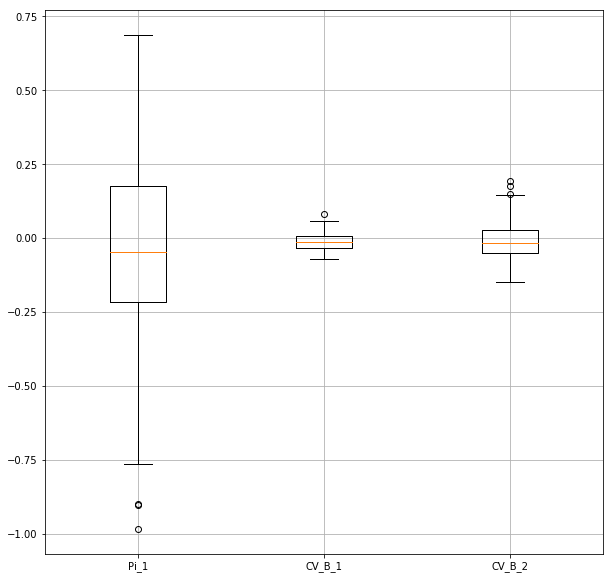
\includegraphics[width=0.4\textwidth]{GM_2d_box.png}
\label{fig:subfig1}}
\qquad
\subfloat[Subfigure 2 list of figures text][d = 8]{
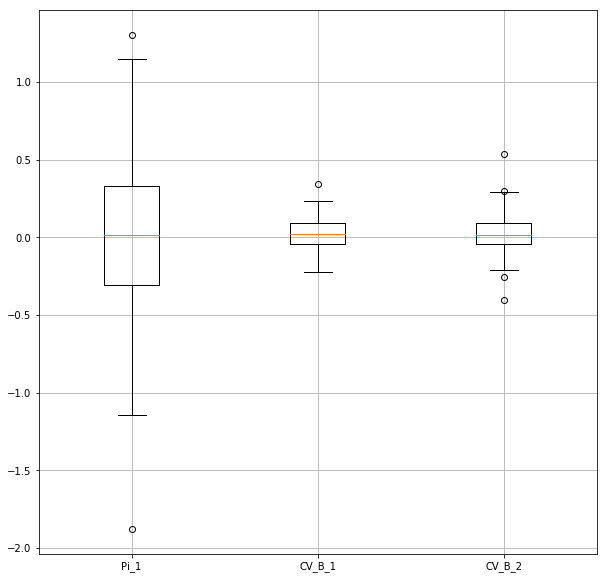
\includegraphics[width=0.4\textwidth]{GM_8d_box.png}
\label{fig:subfig2}}
\caption{Gaussian mixture boxplot}
\end{figure}

\begin{figure}[h]
\centering
\subfloat[Subfigure 1 list of figures text][d = 2]{
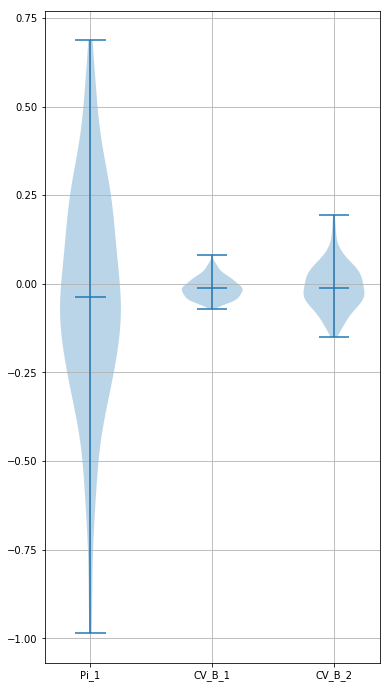
\includegraphics[width=0.4\textwidth]{GM_2d_violin.png}
\label{fig:subfig1}}
\qquad
\subfloat[Subfigure 2 list of figures text][d = 8]{
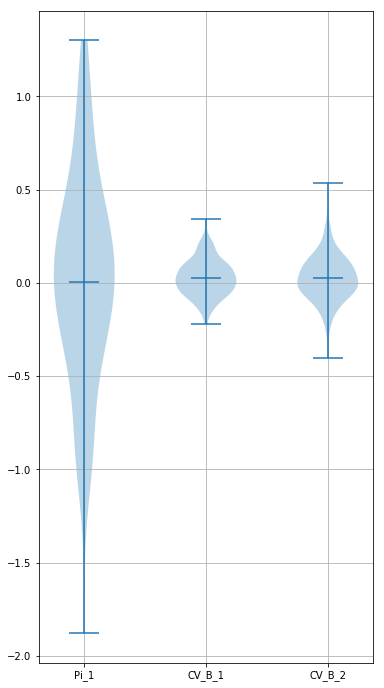
\includegraphics[width=0.4\textwidth]{GM_8d_violin.png}
\label{fig:subfig2}}
\caption{Gaussian mixture violinplot}
\end{figure}

\begin{enumerate}
    \item $d =2, f(x) = x_1 + x_2$
    \begin{enumerate}
    \item Algorithm 1: $n = 1000,N_{train} = 100, \Psi = \{\text{polinomials max}_\text{deg} = 3\}, K =2, \tilde{n} = 100$\\
    K = 1: 109.1 (0.0929643537005 -> 0.000837575184641)\\
    K = 2: 107.1 (0.0929643537005 -> 0.000852084051565)
    
    \item Algorithm 2 :$n = 1000,N_{train} = 1000, \Psi = \{\text{polinomials max}_\text{deg} = 2\}, K =2, \tilde{n} = 60$\\
    K = 1 : 23.34 (0.0929643537005 -> 0.003982653841986601)\\
    K = 2 : 24.76 (0.0929643537005 -> 0.003753718582081946)
    \end{enumerate}
    \item $d =8, f(x) = \sum_{i=1}^d x_i$
    \begin{enumerate}
        
    \item Algorithm 1 $n = 1000,N_{train} = 50, \Psi = \{\text{polinomials max}_\text{deg} = 1\}, K =1, \tilde{n} = 100$\\
    K = 1 : 33.2 (0.3247338706361704 -> 0.00978211277392896)
    
    \item Algorithm 2 $n = 1000,N_{train} = 1000, \Psi = \{\text{polinomials max}_\text{deg} = 1\}, K =1, \tilde{n} = 60$\\
    K = 1 : 20.1 (0.3247338706361704 -> 0.016168075573709376)
    \end{enumerate}
\end{enumerate}

\section{Experiment 2. Binary Logistic regression}

Training set: $\left\{ (X_i, Y_i)\right\}_{i=1,..,n}$, $X_i \in \mathbb{R}^p$ and $Y_i \in \left\{ 0,1\right\}$

\[ r(\theta, x) = \mathbb{P} (Y_i = 1, X_i = x) = \frac{e^{\theta^T x}}{(1 + e^{\theta^Tx})}\]

Let $\pi_0$ is prior probability density on $\theta$, which is Gaussian with zero mean and covariance matrix proportional to the inverse of the Gram matrix $\mathbf{\Sigma}_X = \frac{1}{n} \sum_{i=1}^n X_i X_i^T$, then posterior:

\[ \pi(\theta) \propto \exp \left\{ -Y^TX\theta - \sum_{i=1}^n\log (1 + e^{-\theta^T X_i}) - \frac{\lambda}{2} \| \mathbf{\Sigma}_X^{1/2}\theta\|_2^2\right\}\]

\[f(\theta) = Y^T X \theta + \sum \log (1 + e^{-\theta^T X_i}) + \lambda/2 \| \mathbf{\Sigma}_X^{1/2}\theta\|_2^2\]

\[\bigtriangledown f(\theta) = X^TY - \sum \frac{X_i}{1 + e^{\theta^T X_i}} + \lambda \mathbf{\Sigma}_X\theta \]



Lipschitz constant: $L_g = 0.1 \|\sum \|AX_i \|_2 AX_iX_i^TA \|_2$

X has been generated from a Rademacher distribution and then normalized to have Euclidean norm equal to one. $Y_i$ was drawn from Bernoulli distribution with parameter $r((1,1,..,1)^T, x)$.

\textbf{Results:}

\begin{figure}[h]
\centering
\subfloat[Subfigure 1 list of figures text][d = 2]{
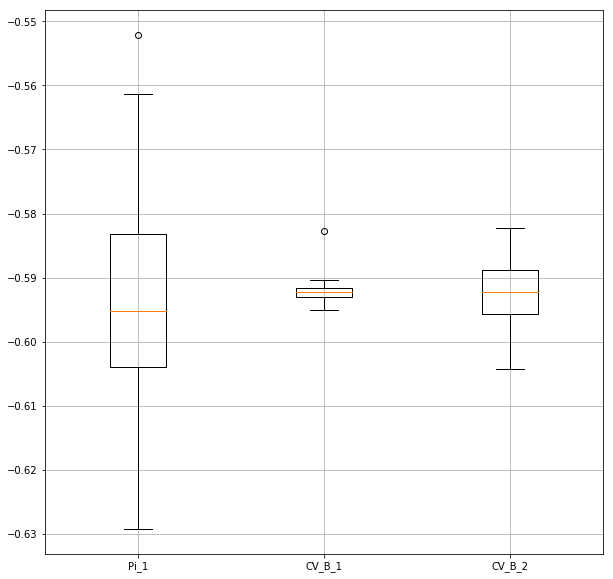
\includegraphics[width=0.4\textwidth]{BLR_2d_box.png}
\label{fig:subfig1}}
\qquad
\subfloat[Subfigure 2 list of figures text][d = 8]{
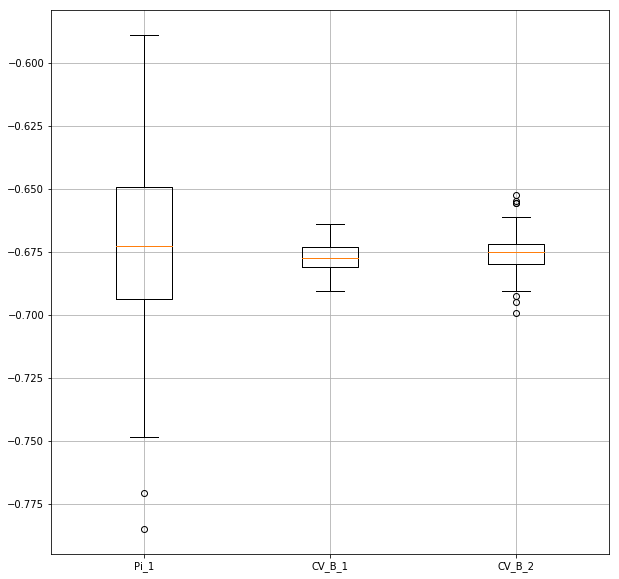
\includegraphics[width=0.4\textwidth]{BLR_8d_box.png}
\label{fig:subfig2}}
\caption{Logistic regression boxplot}
\end{figure}

\begin{figure}[h]
\centering
\subfloat[Subfigure 1 list of figures text][d = 2]{
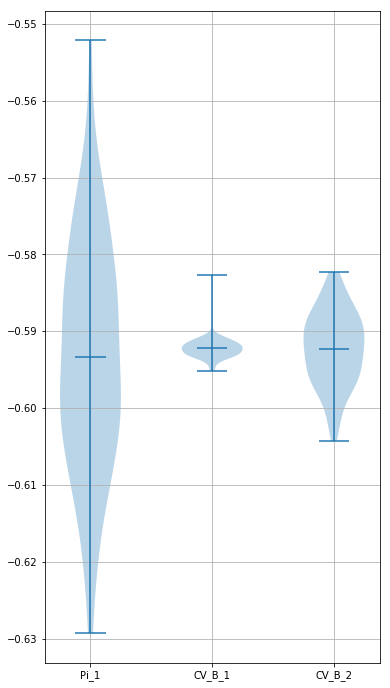
\includegraphics[width=0.4\textwidth]{BLR_2d_violin.png}
\label{fig:subfig1}}
\qquad
\subfloat[Subfigure 2 list of figures text][d = 8]{
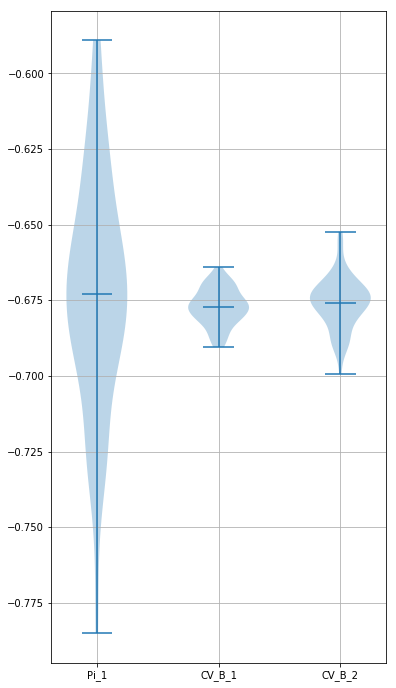
\includegraphics[width=0.4\textwidth]{BLR_8d_violin.png}
\label{fig:subfig2}}
\caption{Logistic regression violinplot}
\end{figure}



\begin{enumerate}
    \item $d =2, f(x) = x_1 + x_2$
    \begin{enumerate}
    \item Algorithm 1: $n = 1000,N_{train} = 50, \Psi = \{\text{polinomials max}_\text{deg} = 3\}, K =1, \tilde{n} = 10$\\
    $K = 1: 117.44 ( 2.18 * 10^{-4} -> 1.858 * 10^{-6} )$\\

    
    \item Algorithm 2 :$n = 1000,N_{train} = 50, \Psi = \{\text{polinomials max}_\text{deg} = 2\}, K =1, \tilde{n} = 3$\\
    $K = 1 : 9.4 (2.18 * 10^{-4} -> 2.32 * 10^{-5})$\\
    
    \end{enumerate}
    \item $d =8, f(x) = \sum_{i=1}^d x_i$
    \begin{enumerate}
        
    \item Algorithm 1 $n = 1000,N_{train} = 50, \Psi = \{\text{polinomials max}_\text{deg} = 1\}, K =1, \tilde{n} = 100$\\
    $K = 1 : 38.67  ( 1.44 * 10^{-3} -> 3.71 * 10^{-5})$
    
    \item Algorithm 2 $n = 1000,N_{train} = 500, \Psi = \{\text{polinomials max}_\text{deg} = 1\}, K =1, \tilde{n} = 3$\\
    $K = 1 : 19.5 ( 1.44 * 10^{-3} -> 7.37 * 10^{-5})$
    \end{enumerate}
\end{enumerate}












\section{CV and ZV}

\subsection{Papamarkou, Mira, Girolami Zero Variance estimator (ZV)}

$$\tilde{f}(x) = f(x) + \frac{H \left[\psi(x) \right]}{\sqrt{\pi(x)}}$$

$$H \left[ \psi(x)\right] = -\frac{1}{2} \Delta_x \left[\psi(x) \right] + \frac{\psi(x)}{2\sqrt{\pi(x)}} \Delta_x \left[ \sqrt{\pi(x)}\right]$$

where $\Delta_x : = \sum_{i = 1}^d \frac{\partial^2}{\partial x^2_i}$

$$\psi(x) = P(x)\sqrt{\pi(x)}$$

$$\tilde{f}(x) = f(x) - \frac{1}{2} \Delta_x \left[ P(x)\right] + \nabla_x \left[ P(x)\right] z(x)$$

$$z(x) = -\frac{1}{2} \nabla_x \left[ln (\pi(x)) \right] = \frac{1}{2} \nabla_x \left[U(x) \right]$$

 First degree polynomials:

$$P(x) = a^T x$$

$$\nabla_x \left[ P(x)\right] = a^T, \quad \Delta_x \left[ P(x)\right] = 0$$

$$\tilde{f}(x) = f(x) + a^T z(x)$$

Optimal $a$:

$$a = - Var^{-1} \left[z(x) \right] * Cov \left[ f(x), z(x)\right]$$

$$\hat{a} = - \hat{Var}^{-1}_{(n)}\left[ z(x)\right] * \hat{Cov}_{(n)} \left[ f(x), z(x)\right]$$

where 

$$\hat{Var}_{(n)}\left[ z(x)\right] = \frac{1}{n-1} \sum_{i=1}^n \left( z(X_i) - \mu\left[ z(X_i) \right]\right) \left( z(X_i) - \mu \left[ z(X_i)\right]\right)^T$$

$$\hat{Cov}_{(n)} \left[ f(x), z(x)\right] = \frac{1}{n-1} \sum_{i=1}^n \left( f(X_i) - \mu \left[ f(X_i)\right]\right)\left( z(X_i) - \mu \left[ z(X_i)\right]\right)$$

$$\pi_n^{ZV_1}(f) = \frac{1}{n} \sum_{k=1}^n \left\{ f(X_k) + \hat{a}^T \nabla U(X_k)\right\}$$

 Second degree polynomials:

$$P(x) = c^T x + \frac{1}{2} x^T B x$$

where $B$ is symmetric

$$\nabla_x \left[ P(x)\right] = (c + Bx)^T, \quad \Delta_x \left[ P(x)\right] = tr(B)$$

$$\tilde{f}(x) = f(x) - \frac{1}{2} tr(B) + (c + Bx)^T z(x)$$

It can be represented as:

$$\tilde(f)(x) = f(x) + a^T w(x)$$

where

$$a = \left[c_1, \dots, c_d, b_{11}, \dots, b_{dd}, b_{12}, \dots, b_{ij}, \dots \right]^T$$

$$w(x) = \left[z_1, \dots, z_d, x_1z_1 - \frac{1}{2}, \dots, x_d z_d - \frac{1}{2}, x_2z_1 + x_1z_2, \dots, x_jz_i + x_i z_j, \dots \right]^T $$

and optimal $a (c,B)$:

$$a^* = - Var \left[w(x) \right]^{-1} Cov \left[f(x), w(x) \right]$$

$$\hat{a}^* = - \hat{Var}_{(n)} \left[w(x) \right]^{-1} \hat{Cov}_{(n)} \left[f(x), w(x) \right]$$

\subsection{N. Brosse Zero-variance estimator (CV)}
define generator: $ \mathfrak{L} \varphi = - <\nabla U, \nabla \varphi> + \Delta \varphi$ 

$\textbf{Note:}\quad \mathfrak{L}\varphi = \frac{2H\left[ \varphi \sqrt{\pi(x)}\right]}{\sqrt{\pi(x)}}$

$$\pi_n^{CV} = \frac{1}{n} \sum_{k=1}^n \left\{ f(X_k) + \mathfrak{L} \left( \hat{\theta}^{*}_n(f)^T \psi (X_k)\right)\right\}$$

optimal $\theta$:

$$\hat{\theta}^{*}_n = H_n^{+} \left[ \frac{1}{n} \sum_{k=1}^n\psi(X_k) \left\{ f(X_k) - \hat{\pi}_n(f)\right\} \right]$$

where
$$ (H_n)_{ij} = \frac{1}{n} \sum_{k=1}^n \left< \nabla \psi_i (X_k), \nabla \psi_j (X_k)\right>$$

 First degree polynomials:

$$\psi = (\psi_1, \dots, \psi_d)$$

$$\psi_i(x) = x_i$$

$$(H_n)_{ij} = \frac{1}{n} \sum_{k=1}^n \left< \nabla \psi_i(X_k), \nabla \psi_j(X_k)\right> = \delta_{ij} \quad \Rightarrow H_n = I$$ 

$$\hat{\theta}^{*}_n (f) = \frac{1}{n} \sum_{k=1}^n X_k \left\{ f(X_k) - \hat{\pi}_n(f)\right\}$$

$$\pi_n^{CV_1} (f) = \frac{1}{n} \sum_{k=1}^n \left\{ f(X_k) - \left< \nabla U(X_k), \hat{\theta}^{*}_n (f)\right>\right\}$$

$$\hat{\theta}^{*}_n (f) = \left[ \hat{Cov}_n(x_1, f(x)), \dots, \hat{Cov}_n(x_d, f(x)) \right]^T$$

 Second degree polynomials:

$$\psi = \left(x_1, \dots, x_d, x_1^2, \dots, x_2^2, x_1x_2, \dots \right)$$

\begin{figure}[h]
\centering
\subfloat[Subfigure 1 list of figures text][d = 2]{
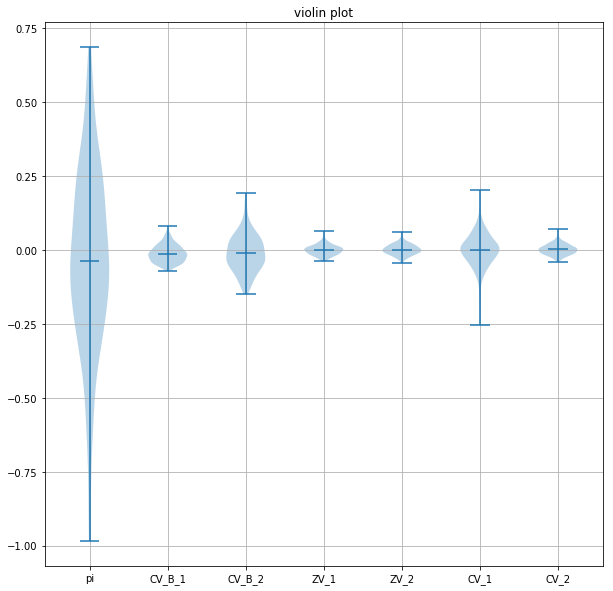
\includegraphics[width=0.4\textwidth]{GM_2d_violin_cv_zv.png}
\label{fig:subfig1}}
\qquad
\subfloat[Subfigure 2 list of figures text][d = 8]{
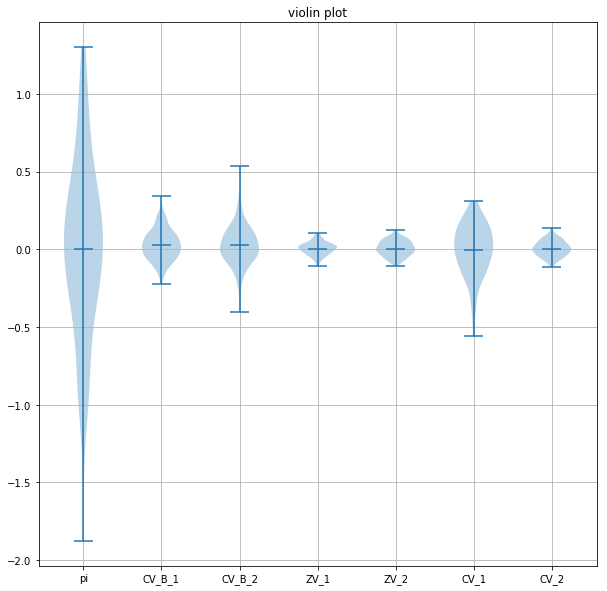
\includegraphics[width=0.4\textwidth]{GM_8d_violin_cv_zv.png}
\label{fig:subfig2}}
\caption{Gaussian mixture violins (cvB1 - algorithm 1, cvB2 - algorithm 2, ZV, CV)}
\end{figure}


\begin{figure}[h]
\centering
\subfloat[Subfigure 1 list of figures text][d = 2]{
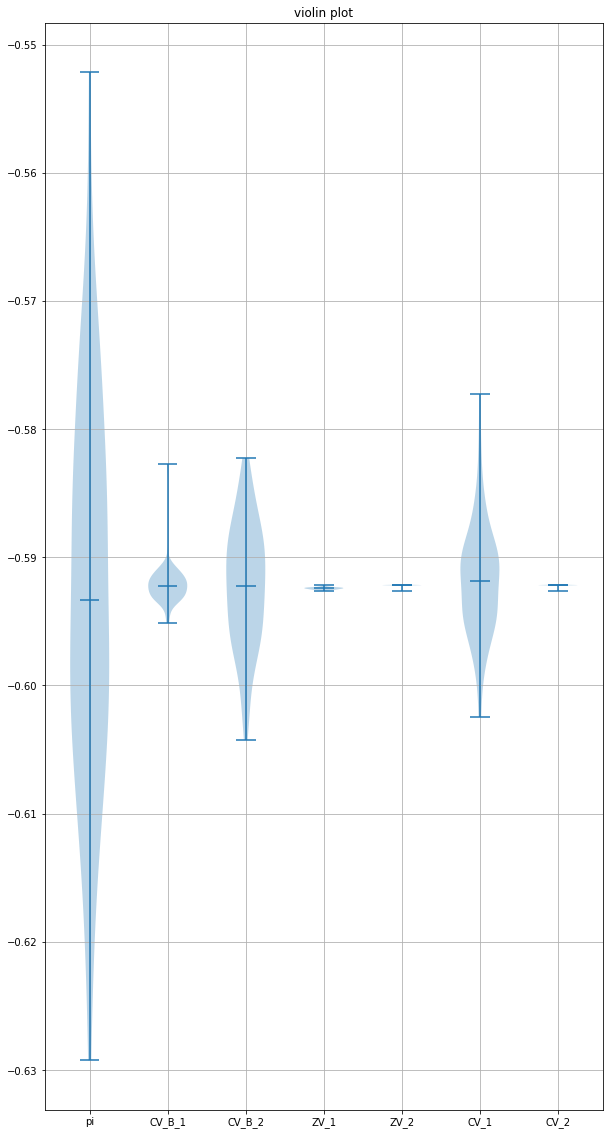
\includegraphics[width=0.4\textwidth]{BLR_2d_violin_cv_zv.png}
\label{fig:subfig1}}
\qquad
\subfloat[Subfigure 2 list of figures text][d = 8]{
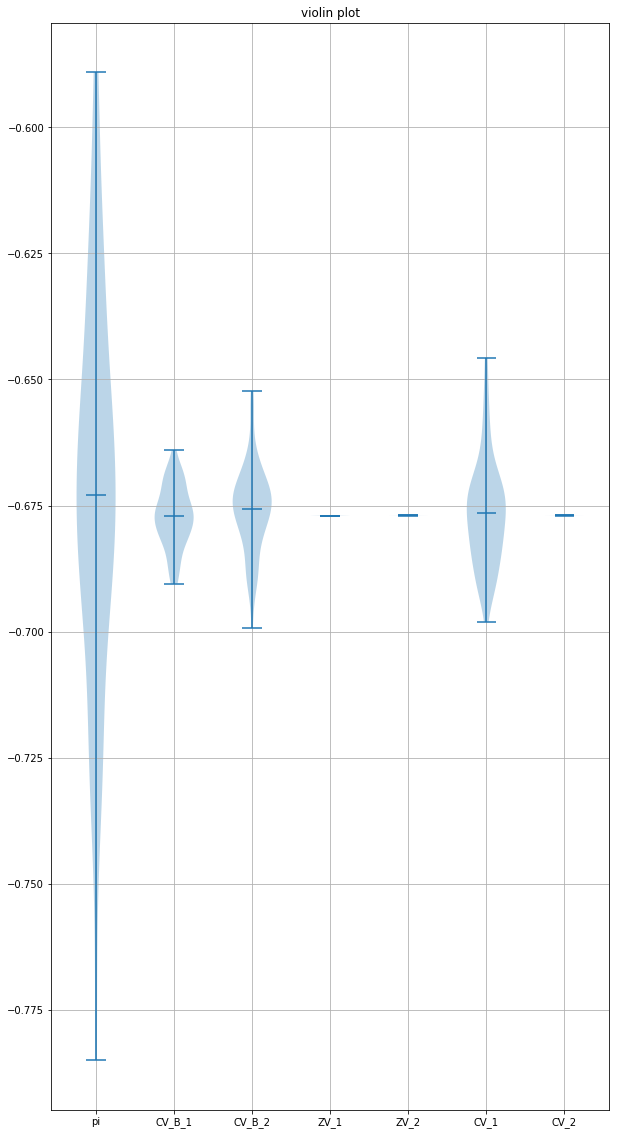
\includegraphics[width=0.4\textwidth]{BLR_8d_violin_cv_zv.png}
\label{fig:subfig2}}
\caption{Logistic regression violins (cvB1 - algorithm 1, cvB2 - algorithm 2, ZV, CV)}
\end{figure}

\section{Conclusion}

Eventually, we have that algorithm 1 is more effective than algorithm 2, however time consumption is considerably bigger. In addition, parameter $\tilde{n}$  in algorithm 1 is less significant and influences on final result slightly ($\tilde{n} = \infty$ doesn't work properly because expectation should convergence to zero with the distance from $X_l$, but we accumulate error and estimation is wrong), while $\tilde{n}$ in algorithm 2 strongly influences on result (requires the right selection to reduce variance, $\tilde{n} = \infty$ doesn't work).  Unfortunately, ZV and CV are more effective (variance reduction and time consumption) than new control variates, however optimisation of algorithm 1 to run trough trajectory by "window" could reduce required number of train trajectory (train by window in repository). Additionaly algorithm from old version of article (algo 1, direct estimation of the coefficient $\bar{a}_{l,k}$) also works with right truncation $\tilde{n}$, but best variance reduction is lower in comparison with algorithm 2 (regression for $\bar{Q}_l$).  
\end{document}